% workflow_figures.tex
% Two publication-quality TikZ figures for the microclCorr package.
%
%   Figure 1 (fig:data_prep)  — Data preparation outside the package
%   Figure 2 (fig:workflow)   — ML pipeline inside the package
%
% Compile with:  pdflatex workflow_figures.tex

\documentclass[a4paper, 11pt]{article}
\usepackage[top=0.5cm, bottom=0.5cm, left=1.0cm, right=1.0cm]{geometry}
\usepackage{tikz}
\usetikzlibrary{shapes.geometric, arrows.meta, positioning, fit, backgrounds, calc}
\usepackage{xcolor}
\usepackage[T1]{fontenc}

%% ── Colour palette ───────────────────────────────────────────────────────────
\definecolor{OutFill} {RGB}{254,243,199}
\definecolor{OutLine} {RGB}{161,100,20}
\definecolor{RFFill}  {RGB}{220,252,231}
\definecolor{RFLine}  {RGB}{22,101,52}
\definecolor{LSTMFill}{RGB}{237,233,254}
\definecolor{LSTMLine}{RGB}{91,33,182}
\definecolor{InfFill} {RGB}{254,226,226}
\definecolor{InfLine} {RGB}{153,27,27}
\definecolor{SelFill} {RGB}{239,246,255}
\definecolor{SelLine} {RGB}{29,78,216}
\definecolor{PrepFill}{RGB}{255,247,237}
\definecolor{PrepLine}{RGB}{234,88,12}

%% ── TikZ styles ──────────────────────────────────────────────────────────────
\tikzset{
  csv/.style={
    cylinder, shape border rotate=90, aspect=0.2,
    draw=gray!60, fill=white, line width=0.5pt,
    align=center, font=\footnotesize\sffamily,
    text width=2.0cm, minimum height=6mm, inner sep=2pt
  },
  steps/.style={
    rectangle, rounded corners=2pt,
    draw=gray!50, fill=white, line width=0.5pt,
    align=left, font=\footnotesize\sffamily,
    inner sep=5pt, text width=7.5cm
  },
  % Generic process box with optional width (default 5 cm)
  proc/.style={
    rectangle, rounded corners=2pt,
    draw=gray!50, fill=white, line width=0.5pt,
    align=center, font=\footnotesize\sffamily,
    inner sep=3pt, text width=#1
  },
  proc/.default=5cm,
  % Wide shared box spanning the full flow
  wide/.style={proc=11.5cm},
  % Coloured group boxes (background layer)
  grpOut/.style ={rectangle, rounded corners=4pt, draw=OutLine,  fill=OutFill,  line width=1pt, inner sep=7pt},
  grpRF/.style  ={rectangle, rounded corners=4pt, draw=RFLine,   fill=RFFill,   line width=1pt, inner sep=7pt},
  grpLSTM/.style={rectangle, rounded corners=4pt, draw=LSTMLine, fill=LSTMFill, line width=1pt, inner sep=7pt},
  grpInf/.style ={rectangle, rounded corners=4pt, draw=InfLine,  fill=InfFill,  line width=1pt, inner sep=7pt},
  grpSel/.style ={rectangle, rounded corners=4pt, draw=SelLine,  fill=SelFill,  line width=1pt, inner sep=7pt},
  grpPrep/.style={rectangle, rounded corners=4pt, draw=PrepLine, fill=PrepFill, line width=1pt, inner sep=7pt},
  arr/.style={->, >=Stealth, line width=0.6pt}
}

% Shorthand for goal/return lines inside boxes
\newcommand{\goal}[1]{{\scriptsize\sffamily Goal: #1}}
\newcommand{\ret}[1] {{\scriptsize\sffamily Returns: #1}}
\newcommand{\addsf}[1]{{\scriptsize\sffamily Adds: #1}}
\newcommand{\savesf}[1]{{\scriptsize\sffamily Saves: #1}}

\begin{document}
\pagestyle{empty}
\hfuzz=3pt   % suppress overfull warnings below 3 pt (< 1 mm, invisible in print)

%% ══════════════════════════════════════════════════════════════════════════════
%%  FIGURE 1 — Data preparation (outside the package)
%% ══════════════════════════════════════════════════════════════════════════════
\begin{figure}[htbp]
\centering
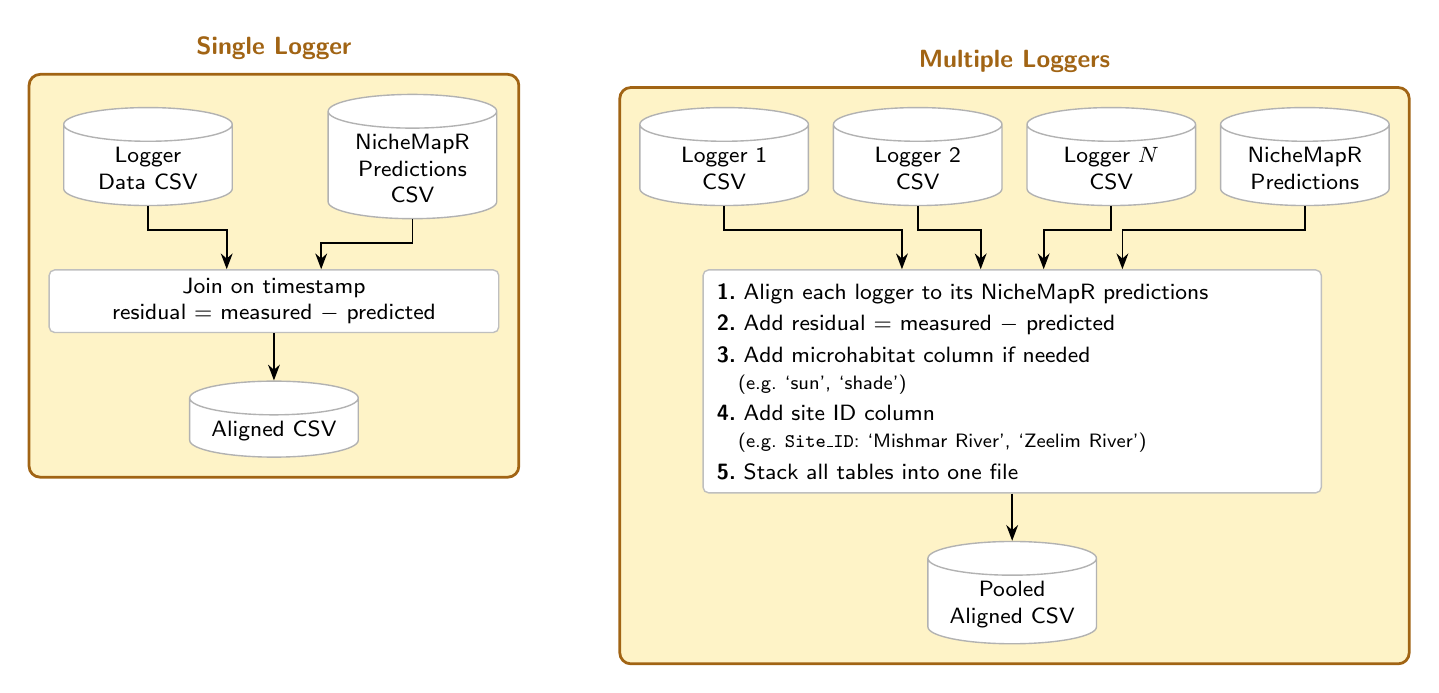
\begin{tikzpicture}[node distance=4mm and 4mm]

  %% ── Single Logger (left) ──────────────────────────────────────────────────
  \node[csv] (lcsv)  {Logger\\Data CSV};
  \node[csv, right=1.2cm of lcsv] (ncsv1) {NicheMapR\\Predictions CSV};

  \node[proc=5.5cm, below=8mm of lcsv, xshift=1.6cm] (join)
    {Join on timestamp\\residual $=$ measured $-$ predicted};

  \node[csv, below=6mm of join] (acsv) {Aligned CSV};

  \draw[arr] (lcsv.south)  -- ++(0,-3mm) -| ([xshift=-6mm]join.north);
  \draw[arr] (ncsv1.south) -- ++(0,-3mm) -| ([xshift= 6mm]join.north);
  \draw[arr] (join) -- (acsv);

  \begin{scope}[on background layer]
    \node[grpOut, fit=(lcsv)(ncsv1)(join)(acsv)] (sg) {};
  \end{scope}
  \node[font=\small\bfseries\sffamily, text=OutLine, above=1.5pt] at (sg.north)
    {Single Logger};

  %% ── Multiple Loggers (right) ──────────────────────────────────────────────
  \node[csv, right=1.8cm of ncsv1] (l1) {Logger 1\\CSV};
  \node[csv, right=3mm  of l1]     (l2) {Logger 2\\CSV};
  \node[csv, right=3mm  of l2]     (ln) {Logger $N$\\CSV};
  \node[csv, right=3mm  of ln]     (nm) {NicheMapR\\Predictions};

  \node[steps, below=8mm of l2, xshift=1.2cm] (stps) {
    \textbf{1.}~Align each logger to its NicheMapR predictions\\[2pt]
    \textbf{2.}~Add residual $=$ measured $-$ predicted\\[2pt]
    \textbf{3.}~Add microhabitat column if needed\\
    \hspace*{0.9em}{\scriptsize(e.g.\ `sun', `shade')}\\[2pt]
    \textbf{4.}~Add site ID column\\
    \hspace*{0.9em}{\scriptsize(e.g.\ \texttt{Site\_ID}: `Mishmar River', `Zeelim River')}\\[2pt]
    \textbf{5.}~Stack all tables into one file
  };

  \node[csv, below=6mm of stps] (pcsv) {Pooled\\Aligned CSV};

  \draw[arr] (l1.south) -- ++(0,-3mm) -| ([xshift=-14mm]stps.north);
  \draw[arr] (l2.south) -- ++(0,-3mm) -| ([xshift= -4mm]stps.north);
  \draw[arr] (ln.south) -- ++(0,-3mm) -| ([xshift=  4mm]stps.north);
  \draw[arr] (nm.south) -- ++(0,-3mm) -| ([xshift= 14mm]stps.north);
  \draw[arr] (stps) -- (pcsv);

  \begin{scope}[on background layer]
    \node[grpOut, fit=(l1)(l2)(ln)(nm)(stps)(pcsv)] (mg) {};
  \end{scope}
  \node[font=\small\bfseries\sffamily, text=OutLine, above=1.5pt] at (mg.north)
    {Multiple Loggers};

\end{tikzpicture}
\caption{\sloppy Data preparation users need to perform outside the \texttt{microclCorr} package.
  First, the user aligns the logger measurements with the Niche\-MapR predictions on
  timestamp and computes the residual (measured minus predicted).
  For a single logger (left), this produces a single aligned CSV file.
  For multiple loggers (right), the user additionally assigns a microhabitat label
  and a site identifier to each row, then concatenates all loggers into one file.
  Both paths produce an aligned CSV that serves as input to the ML pipeline
  (Fig.\,\ref{fig:workflow}).}
\label{fig:data_prep}
\end{figure}


%% ══════════════════════════════════════════════════════════════════════════════
%%  FIGURE 2 — ML pipeline (inside the package)
%% ══════════════════════════════════════════════════════════════════════════════
\begin{figure}[htbp]
\centering
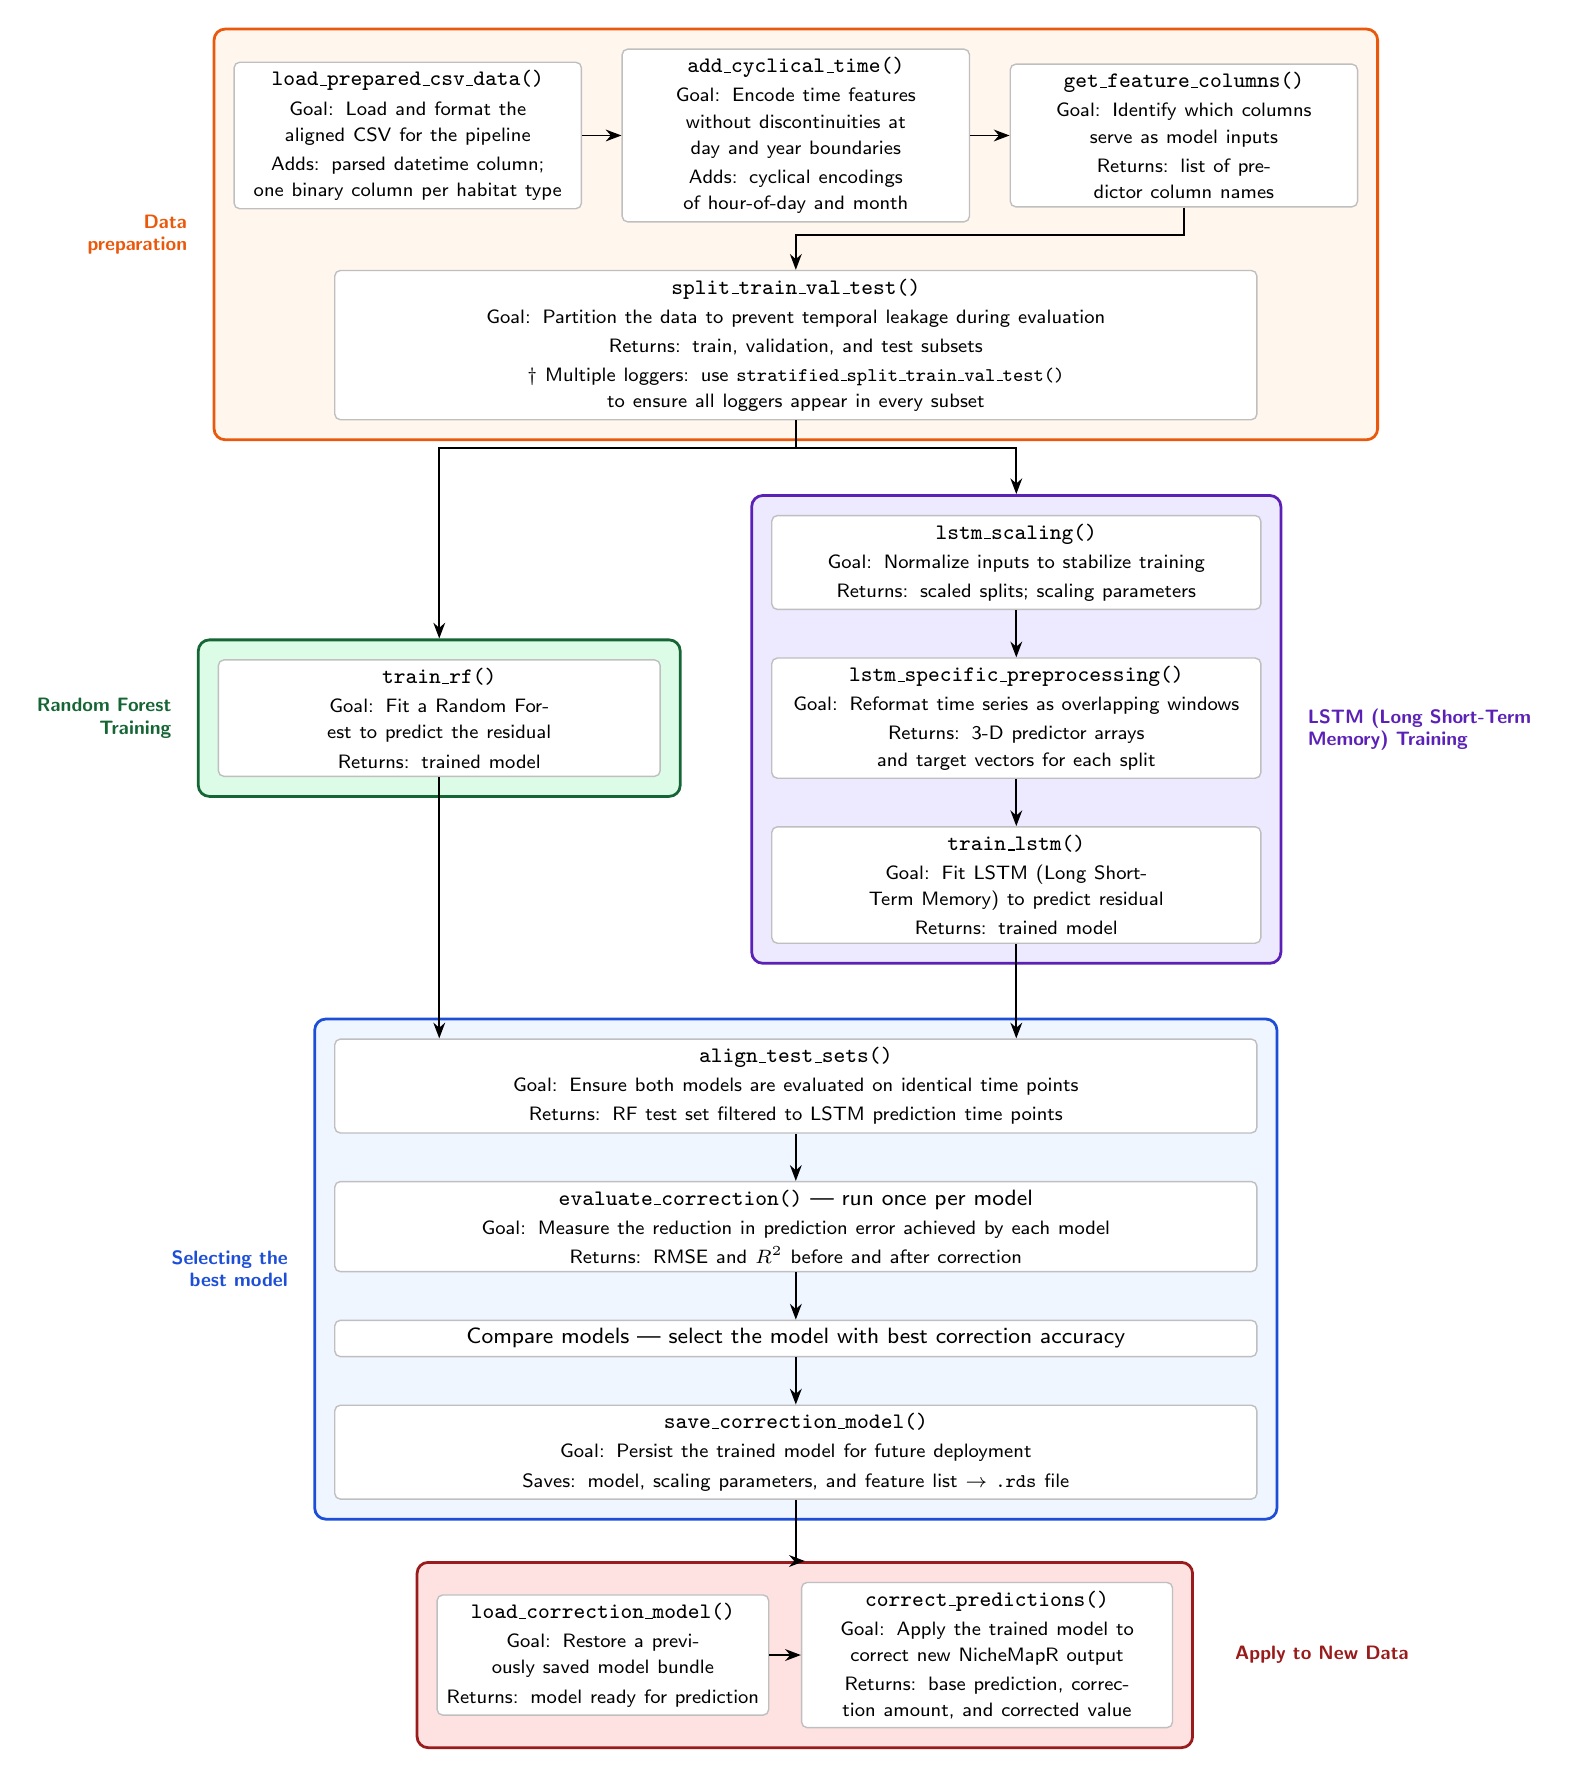
\begin{tikzpicture}[node distance=6mm]

  %% ── Shared top (Horizontal Layout for Data Preparation) ────────────────────
  \node[proc=4.2cm] (cycl)
    {\texttt{add\_cyclical\_time()}\\[1pt]
     \goal{Encode time features without discontinuities at day and year boundaries}\\[1pt]
     \addsf{cyclical encodings of hour-of-day and month}};

  \node[proc=4.2cm, left=5mm of cycl] (load)
    {\texttt{load\_prepared\_csv\_data()}\\[1pt]
     \goal{Load and format the aligned CSV for the pipeline}\\[1pt]
     \addsf{parsed datetime column; one binary column per habitat type}};

  \node[proc=4.2cm, right=5mm of cycl] (feat)
    {\texttt{get\_feature\_columns()}\\[1pt]
     \goal{Identify which columns serve as model inputs}\\[1pt]
     \ret{list of predictor column names}};

  \node[wide, below=of cycl] (splt)
    {\texttt{split\_train\_val\_test()}\\[1pt]
     \goal{Partition the data to prevent temporal leakage during evaluation}\\[1pt]
     \ret{train, validation, and test subsets}\\[1pt]
     {\scriptsize\sffamily$\dagger$~Multiple loggers: use
      \texttt{stratified\_split\_train\_val\_test()} to ensure all loggers appear in every subset}};

  \draw[arr] (load) -- (cycl);
  \draw[arr] (cycl) -- (feat);
  \draw[arr] (feat.south) -- ++(0,-3.5mm) -| (splt.north);

  \begin{scope}[on background layer]
    \node[grpPrep, fit=(load)(cycl)(feat)(splt)] (prepg) {};
  \end{scope}
  % Label on the side of the Prep box
  \node[font=\scriptsize\bfseries\sffamily, text=PrepLine, anchor=east, align=right]
    at ([xshift=-2mm]prepg.west) {Data\\preparation};

  %% ── LSTM branch (right) ────────────────────────────────────────────────────
  \node[proc=6.0cm, below=12mm of splt, xshift=2.8cm] (scl)
    {\texttt{lstm\_scaling()}\\[1pt]
     \goal{Normalize inputs to stabilize training}\\[1pt]
     \ret{scaled splits; scaling parameters}};

  \node[proc=6.0cm, below=of scl] (win)
    {\texttt{lstm\_specific\_preprocessing()}\\[1pt]
     \goal{Reformat time series as overlapping windows}\\[1pt]
     \ret{3-D predictor arrays and target vectors for each split}};

  \node[proc=6.0cm, below=of win] (ltt)
    {\texttt{train\_lstm()}\\[1pt]
     \goal{Fit LSTM (Long Short-Term Memory) to predict residual}\\[1pt]
     \ret{trained model}};

  \draw[arr] (scl) -- (win);
  \draw[arr] (win) -- (ltt);

  \begin{scope}[on background layer]
    \node[grpLSTM, fit=(scl)(win)(ltt)] (lstmg) {};
  \end{scope}
  % Label on the side of the LSTM box
  \node[font=\scriptsize\bfseries\sffamily, text=LSTMLine, anchor=west, align=left]
    at ([xshift=2mm]lstmg.east) {LSTM (Long Short-Term\\Memory) Training};

  %% ── RF branch (left) ───────────────────────────────────────────────────────
  \node[proc=5.4cm, left=1.4cm of win] (rft)
    {\texttt{train\_rf()}\\[1pt]
     \goal{Fit a Random Forest to predict the residual}\\[1pt]
     \ret{trained model}};

  \begin{scope}[on background layer]
    \node[grpRF, fit=(rft)] (rfg) {};
  \end{scope}
  % Label on the side of the RF box
  \node[font=\scriptsize\bfseries\sffamily, text=RFLine, anchor=east, align=right]
    at ([xshift=-2mm]rfg.west) {Random Forest\\Training};

  %% ── Arrows: split → branches ───────────────────────────────────────────────
  \draw[arr] (splt.south) -- ++(0,-3.5mm) -| (rfg.north);
  \draw[arr] (splt.south) -- ++(0,-3.5mm) -| (lstmg.north);

  %% ── Shared bottom ──────────────────────────────────────────────────────────
  % algn centred below both branches (xshift corrects for ltt being off-centre)
  \node[wide, below=12mm of ltt, xshift=-2.8cm] (algn)
    {\texttt{align\_test\_sets()}\\[1pt]
     \goal{Ensure both models are evaluated on identical time points}\\[1pt]
     \ret{RF test set filtered to LSTM prediction time points}};

  % Straight vertical arrows from each branch to align
  \draw[arr] (rft.south) -- (rft.south |- algn.north);
  \draw[arr] (ltt.south) -- (ltt.south |- algn.north);

  \node[wide, below=of algn] (eval)
    {\texttt{evaluate\_correction()} --- run once per model\\[1pt]
     \goal{Measure the reduction in prediction error achieved by each model}\\[1pt]
     \ret{RMSE and $R^{2}$ before and after correction}};

  \node[wide, below=of eval] (cmp)
    {Compare models --- select the model with best correction accuracy};

  \node[wide, below=of cmp] (sav)
    {\texttt{save\_correction\_model()}\\[1pt]
     \goal{Persist the trained model for future deployment}\\[1pt]
     \savesf{model, scaling parameters, and feature list $\to$ \texttt{.rds} file}};

  \draw[arr] (algn) -- (eval);
  \draw[arr] (eval) -- (cmp);
  \draw[arr] (cmp)  -- (sav);

  \begin{scope}[on background layer]
    \node[grpSel, fit=(algn)(eval)(cmp)(sav)] (selg) {};
  \end{scope}
  % Label on the side of the Sel box
  \node[font=\scriptsize\bfseries\sffamily, text=SelLine, anchor=east, align=right]
    at ([xshift=-2mm]selg.west) {Selecting the\\best model};

  %% ── Inference box ──────────────────────────────────────────────────────────
  \node[proc=4.0cm, below=12mm of sav, xshift=-2.45cm] (ldm)
    {\texttt{load\_correction\_model()}\\[1pt]
     \goal{Restore a previously saved model bundle}\\[1pt]
     \ret{model ready for prediction}};

  \node[proc=4.5cm, right=4mm of ldm] (prd)
    {\texttt{correct\_predictions()}\\[1pt]
     \goal{Apply the trained model to correct new NicheMapR output}\\[1pt]
     \ret{base prediction, correction amount, and corrected value}};

  \draw[arr] (ldm) -- (prd);

  \begin{scope}[on background layer]
    \node[grpInf, fit=(ldm)(prd)] (infg) {};
  \end{scope}
  % Label to the RIGHT of the inference box (horizontal)
  \node[font=\scriptsize\bfseries\sffamily, text=InfLine, anchor=west]
    at ([xshift=4mm]infg.east) {Apply to New Data};

  \draw[arr] (sav.south) -- ++(0,-6mm) |- (infg.north);

\end{tikzpicture}
\caption{Machine learning pipeline implemented within \texttt{microclCorr}.
  First, the aligned CSV is loaded, cyclical time features are added, predictor
  columns are identified, and the data are split into training, validation, and test subsets.
  Next, the data are passed to two parallel training branches:
  a Random Forest (left) and a Long Short-Term Memory (LSTM) network (right);
  steps marked with $\dagger$ differ for the pooled (multiple-logger) scenario.
  Next, both models are evaluated on identical test time points and compared to select the best correction accuracy.
  Finally, the best-performing model is saved and can be applied to correct new predictions.}
\label{fig:workflow}
\end{figure}

\end{document}
